\documentclass[a4paper,12pt]{article}
\usepackage[margin=1in]{geometry}

\usepackage[T2A]{fontenc}			% кодировка
\usepackage[utf8]{inputenc}			% кодировка исходного текста
\usepackage[english,russian]{babel}	% локализация и переносы
\usepackage{graphicx}                % Математика
\usepackage{amsmath,amsfonts,amssymb,amsthm,mathtools} 
\usepackage{mathtext}
\usepackage[T2A]{fontenc}
\usepackage[utf8]{inputenc}

\usepackage{wasysym}
\usepackage{placeins}

%Заговолок
\author{Бичина Марина 
группа Б04-005 1 курса ФЭФМ}
\title{}
\date{}


\begin{document} % начало документа

\begin{center}
\begin{Large}
{ Марина Б04-005, Лабораторная работа №.3.2.3}
\end{Large}
\end{center}
\paragraph{Цель работы:} 

Исследование резонанса токов в параллельном колебательном контуре с
изменяемой ёмкостью, включающее получение амплитудно-частотных и фазово-частотных
характеристик, а также определение основных параметров контура.

\paragraph{Оборудование:}
\begin{enumerate}
\itemsep0em
\item генератор сигналов
\item источник тока, нагруженный на параллельный колебательный контур с переменной ёмкостью
\item двухлучевой осциллограф
\item цифровые вольтметры
\end{enumerate}

\FloatBarrier

\paragraph{Теоретическая справка:}

\begin{figure}
\centering
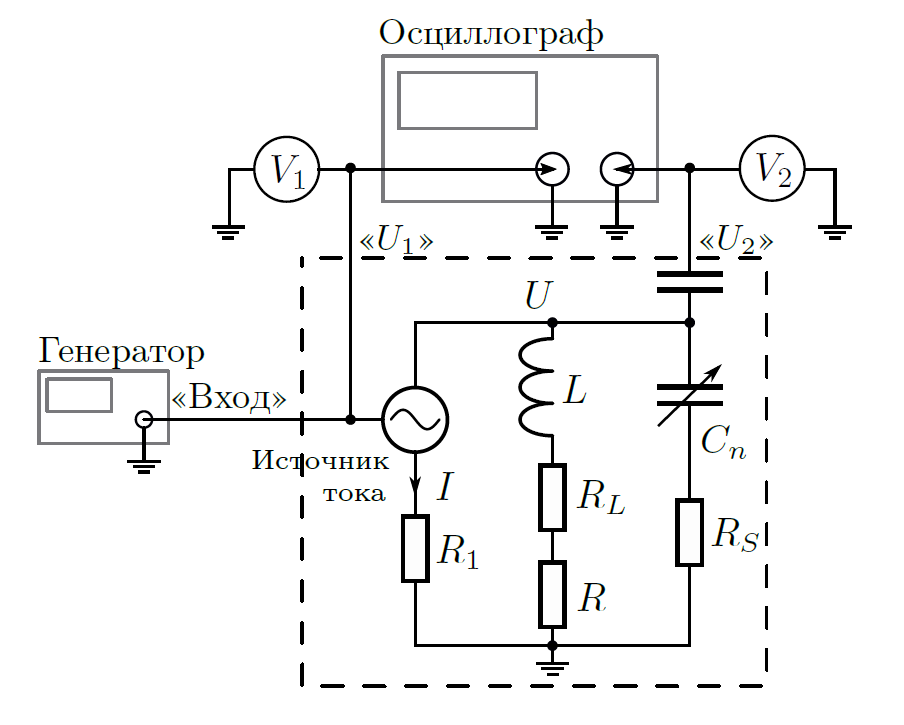
\includegraphics[width=0.5\textwidth]{setup.png}
\caption{Блок-схема экспериментального стенда}
\end{figure}

\paragraph{}

Напряжение $\mathcal{E} = \mathcal{E}_0 \cos (\omega t + \varphi_0)$ от генератора поступает на вход источника тока. Переменное напряжение на сопротивлении $R_1$ в используемой схеме равно напряжению на выходе генератора и совпадает с ним по фазе, то есть:

\begin{equation}
I = \frac{\mathcal{E}}{R_1} = I_0 \cos (\omega t + \varphi_0), \;\;\; I_0 = \frac{\mathcal{E}_0}{R_1}.
\end{equation}

\noindent Выражения для импеданса ёмкостной и индуктивной ветви параллельного контура:

\begin{equation}
Z_c = R_s - \frac{i}{\omega C}, \;\;\; Z_L = R + R_L + i\omega L.
\end{equation}

\begin{figure}
\centering
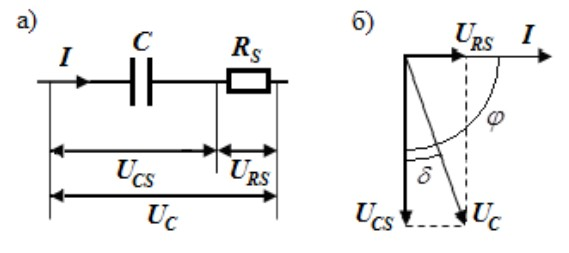
\includegraphics[width=0.5\textwidth]{setup2.png}\
\caption{Последовательная эквивалентная схема конденсатора с потерями}
\end{figure}

Комплексные амплитуды токов в ёмкостной и индуктивной ветвях контура, а также напряжения на контуре при нулевой начальной фазе внешнего тока удобно представить в виде:

\begin{equation}
\begin{array}{llll}
\hat{I}_C = QI_0 \frac{\omega}{\omega_0}\frac{e^{i \varphi_C}}{\sqrt{1 + (\tau \Delta \omega)^2}}
&
, 
&
\varphi_C = \frac{\pi}{2} - \frac{R + R_L}{\rho} - \arctg (\tau \Delta \omega)
&
,
\\
\hat{I}_L = QI_0 \frac{\omega}{\omega_0}\frac{e^{i \varphi_L}}{\sqrt{1 + (\tau \Delta \omega)^2}}&
, 
&
\varphi_L = - \frac{\pi}{2} + \delta - \arctg (\tau \Delta \omega)
&
,
\\	
\hat{U} = Q\rho I_0 \frac{e^{i \varphi_U}}{\sqrt{1 + (\tau \Delta \omega)^2}}
&
, 
&
\varphi_U = - \frac{\omega_0}{\omega} \frac{R + R_L}{\rho} + \delta - \arctg (\tau \Delta \omega)
&
.
\\	
\end{array}
\end{equation}

При резонансе модули комплексных амплитуд, их фазы и производные фаз по циклической частоте принимают вид:

\begin{equation}
\begin{array}{llll}
I_C(\omega_0) = QI_0 & , & \varphi_C(\omega_0) = \frac{\pi}{2} - \frac{R + R_L}{\rho} & , \\

I_L(\omega_0) = QI_0 & , & \varphi_L(\omega_0) = - \frac{\pi}{2} + \delta & , \\

U(\omega_0) = Q\rho I_0 = Q^2 R_\Sigma I_0  & , & \varphi_U (\omega_0) = -  \frac{R + R_L}{\rho} + \delta & , \\

\varphi'_C (\omega_0) = \varphi'_L (\omega_0) = \varphi'_U(\omega_0) = -\tau . \\

\end{array}
\end{equation}

\paragraph{Параметры установки:} $R = 3.5$ Ом, $R_1 = 1008$ Ом.


\paragraph{Ход работы:}
\begin{enumerate}
\itemsep0em
\item Проведём измерения для контуров с различными ёмкостями (таблица 1)


\begin{table}[h]
\centering
\footnotesize
\begin{tabular}{|llll|l|l|l|l|l|l|l|}
\hline
\multicolumn{1}{|l|}{$C_n$,нФ} & \multicolumn{1}{l|}{$f_{0n}$,кГц} & \multicolumn{1}{l|}{$U$,В} & $E$,В & $L$, мкГн & $\rho$,Ом & $Z_\text{рез}$,Ом & $Q$ & $R_\Sigma$,Ом & $R_{S \max}$,Ом & $R_L$,Ом \\ \hline
\multicolumn{1}{|l|}{25.10} & \multicolumn{1}{l|}{32.00} & \multicolumn{1}{l|}{1.23} & 0.25 & 986.52 & 198.25 & 4959.36 & 25.02 & 7.93 & 0.20 & 4.23 \\
\multicolumn{1}{|l|}{33.20} & \multicolumn{1}{l|}{27.70} & \multicolumn{1}{l|}{1.15} & 0.25 & 995.37 & 173.15 & 4636.80 & 26.78 & 6.47 & 0.17 & 2.79 \\
\multicolumn{1}{|l|}{47.30} & \multicolumn{1}{l|}{23.20} & \multicolumn{1}{l|}{0.83} & 0.25 & 995.96 & 145.11 & 3346.56 & 23.06 & 6.29 & 0.15 & 2.65 \\
\multicolumn{1}{|l|}{57.40} & \multicolumn{1}{l|}{21.30} & \multicolumn{1}{l|}{0.72} & 0.25 & 973.67 & 130.24 & 2903.04 & 22.29 & 5.84 & 0.13 & 2.21 \\
\multicolumn{1}{|l|}{67.50} & \multicolumn{1}{l|}{19.50} & \multicolumn{1}{l|}{0.59} & 0.25 & 987.89 & 120.98 & 2378.88 & 19.66 & 6.15 & 0.12 & 2.53 \\
\multicolumn{1}{|l|}{82.70} & \multicolumn{1}{l|}{17.70} & \multicolumn{1}{l|}{0.50} & 0.25 & 978.65 & 108.78 & 2016.00 & 18.53 & 5.87 & 0.11 & 2.26 \\
\multicolumn{1}{|l|}{101.60} & \multicolumn{1}{l|}{15.90} & \multicolumn{1}{l|}{0.42} & 0.25 & 897.17 & 98.57 & 1693.44 & 17.18 & 5.74 & 0.10 & 2.14 \\ \hline
\multicolumn{4}{|l|}{Среднее значение} & 986.46 &  &  &  &  &  & 2.69 \\ \hline
\multicolumn{4}{|l|}{Среднеквадратичная погрешность} & 3.07 &  &  &  &  &  & 0.27 \\ \hline
\end{tabular}
\caption{Результаты измерений}
\end{table}

\begin{equation}
\begin{array}{lllllll}
\rho = \sqrt{\frac{L}{C}} & , & Z_\text{рез} = \frac{U}{I_0} = \frac{UR_1}{E} & , & Q = \frac{Z_\text{рез}}{\rho} & , \\
R_\Sigma = \frac{Z_\text{рез}}{Q^2} & , & R_{S \max} = \tg \frac{\delta}{\omega C} & , & R_L = R_\Sigma - R - R_s & . \\

\end{array}
\end{equation}

\item Снимем АЧХ для двух контуров 3 и 7 в размерных и безразмерных координатах (рис. 3.)

\begin{figure}[h]
\centering
\begin{minipage}[h]{0.49\textwidth}
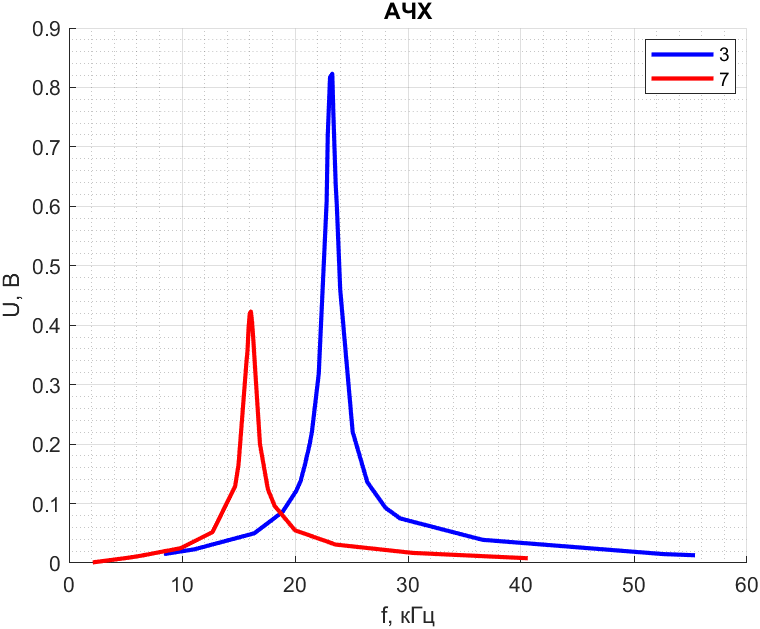
\includegraphics[width=\textwidth]{afc_1.png}
\center{а) в размерных величинах}
\end{minipage}
\begin{minipage}[h]{0.49\textwidth}
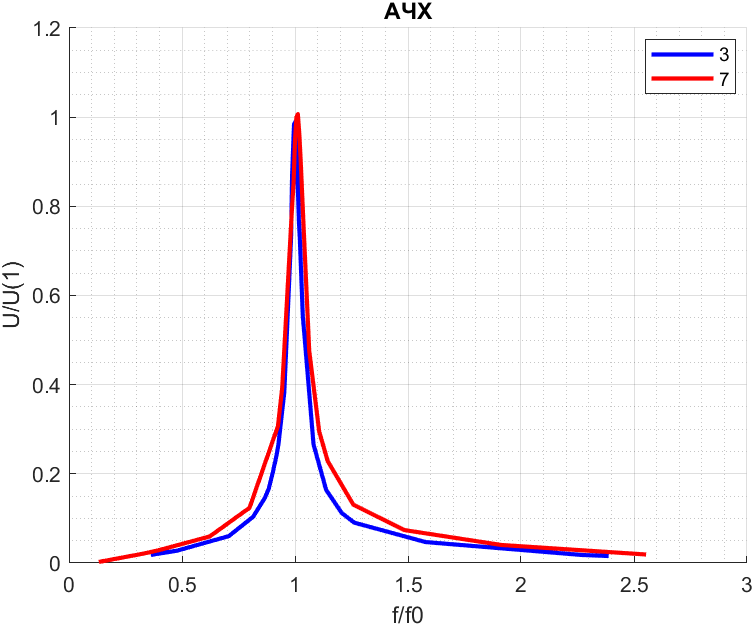
\includegraphics[width=\textwidth]{afc_2.png}
\center{б) в безразмерных величинах}
\end{minipage}
\caption{АЧХ 3 и 7 контуров}
\end{figure}

Резонанс для контура 7 достигается на меньших частотах, чем у контура 3. Однако, в безразмерных координатах пики АЧХ двух контуров совпадают.

Графически определяем добротность: $Q_3=25$ ; $Q_7=15.6$ . Полученные значения сходятся с значениями в таблице 1.

\item Построим ФЧХ контуров (рис. 4).

\begin{figure}[h]
\centering
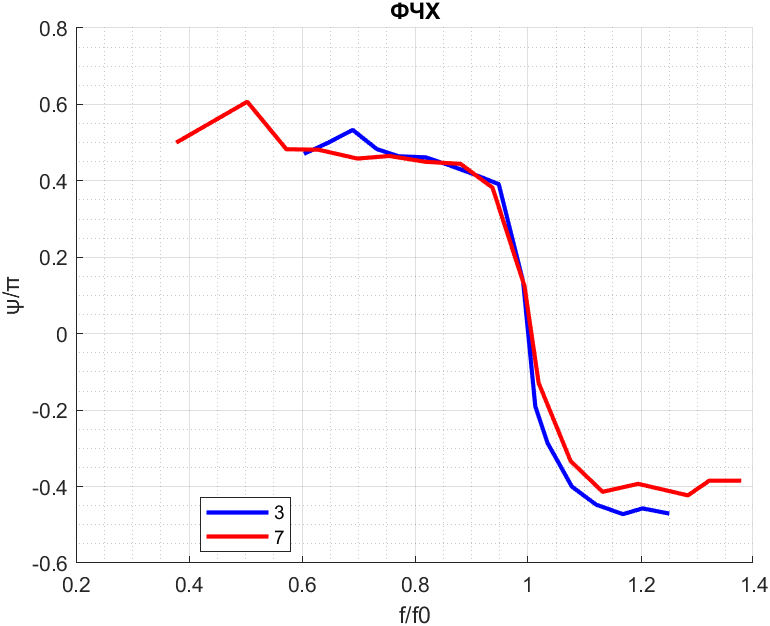
\includegraphics[width=0.7\textwidth]{pfc.png}
\caption{ФЧХ контуров}
\end{figure}

По формуле $Q = \frac{1}{2} \frac{d\varphi_U(x)}{dx}$ определим добротность по ФЧХ: $Q_3 = 7.4, \; Q_7 = 4.25$.

\item По данным из таблицы 1 Построим график зависимости $RL (f0)$. (рис. 5)

\begin{figure}[h]
\centering
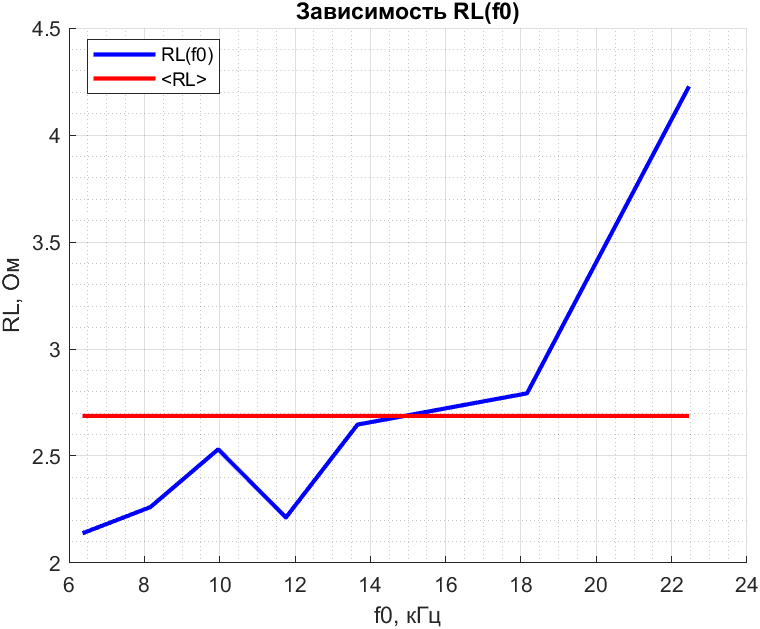
\includegraphics[width=0.7\textwidth]{rl.png}
\caption{Зависимость активного сопротивления от резонансной частоты}
\end{figure}

\FloatBarrier

\end{enumerate}
\paragraph{Выводы:}
\begin{enumerate}
\item В ходе лабораторной работы мы исследовали резонанс токов в параллельном колебательном контуре с изменяемой ёмкостью, в ходе изучения получили амплитудно-частотные и фазово-частотные характеристики, а также определили основные параметры контура.

\item Мы вычислили значение добротности контура тремя различными способами, получили значения:

\[
\begin{array}{lllllll}
Q_3^{табл} = 23.06 & , & Q_3^{АЧХ} = 25 & , & Q_3^{ФЧХ} = 7.4 & ; \\
Q_7^{табл} = 5.79 & , & Q_7^{АЧХ} = 15.6 & , & Q_7^{ФЧХ} = 4.25 & . \\
\end{array}
\]

Для контура 3 ближе к теоретическому значению оказалась добротность, полученная
графически при помощи АЧХ, а для контура 7 — при помощи ФЧХ.

\item Также была изучена зависимость активного сопротивления катушки индуктивности.
Можно заметить, что активное сопротивление увеличивается при увеличении частоты, это
может быть связано с потерями на катушке при перемагничивании сердечника, и с потерями,
обусловленными возникновением вихревых токов.

\end{enumerate}
\end{document}